% Hardware
%
The task description for this project as seen in appendix \autoref{app:Aufgabenstellung} requires the following hardware changes:
%
\begin{itemize}%
    \item Optimization of size and weight %
    \item Optimization for outdoor use%
    \item Usage of more powerful processor with more memory and RNG or encryption support %
    \item SWD/JTAG debugging interface%
    \item UART hardware flow control
    \item On-board SD card (regular or micro)
\end{itemize}% \\
%
There are several options on how to proceed with the implementation. The pro and cons of these choices are listed in this chapter, followed by the chosen solution and its execution.
%
%
%
\section{Hardware Redesign Options}
The hardware Andreas Albisser designed is working as expected. The desired modifications as listed in the task description are merely optimizations. Only the replacement of the Teensy 3.1 is absolutely required for this project because software will later be written for a specific micro controller. \\
Therefore there are two options on how to proceed.\\
%
\begin{itemize}
    \item Redesign entire hardware for/with a new processor.
    \item Redesign hardware step by step, starting with just an adapter board to use existing hardware with new micro controller.
\end{itemize}
%
\subsection{Complete Hardware Redesign}
A redesign of the entire hardware requires careful component selection, adaption of the schematic and footprints and redesign of the PCB. \\
Changes for the next complete hardware redesign include:
\begin{itemize}
    \item New RS232 level to TTL level converter with more inputs to convert hardware flow control pins (CTS/RTS) as well. The converter currently used has no more free pins available. Alternatively add more components of the already used converter for the hardware flow control signals.
    \item A way to switch between RS232 level and TTL level for all serial interfaces accessible to the user to allow for TTL modems to be connected as well.
    \item More powerful micro controller with support for encryption and SD card slot.
    \item Hardware debugging interface.
    \item Use of different connector as user interface, with more pins to include hardware flow control signals.
\end{itemize}
Implementing all these changes would require about three weeks, followed by one week of manufacturing and one week of assembly. In case of a faulty hardware, it would be extremely difficult start with the software implementation because there is no hardware to work with and no way to work standalone. In this case, producing a second version of the hardware would take up a considerable amount of time because of manufacturing time, assembly and testing.\\
There is simply not enough time to redesign the entire hardware in the scope of this project.\\
A possible project plan for this scenario can be found in \autoref{Project plan complete HW redesign}:\\
\begin{figure}[H]
    \centering
    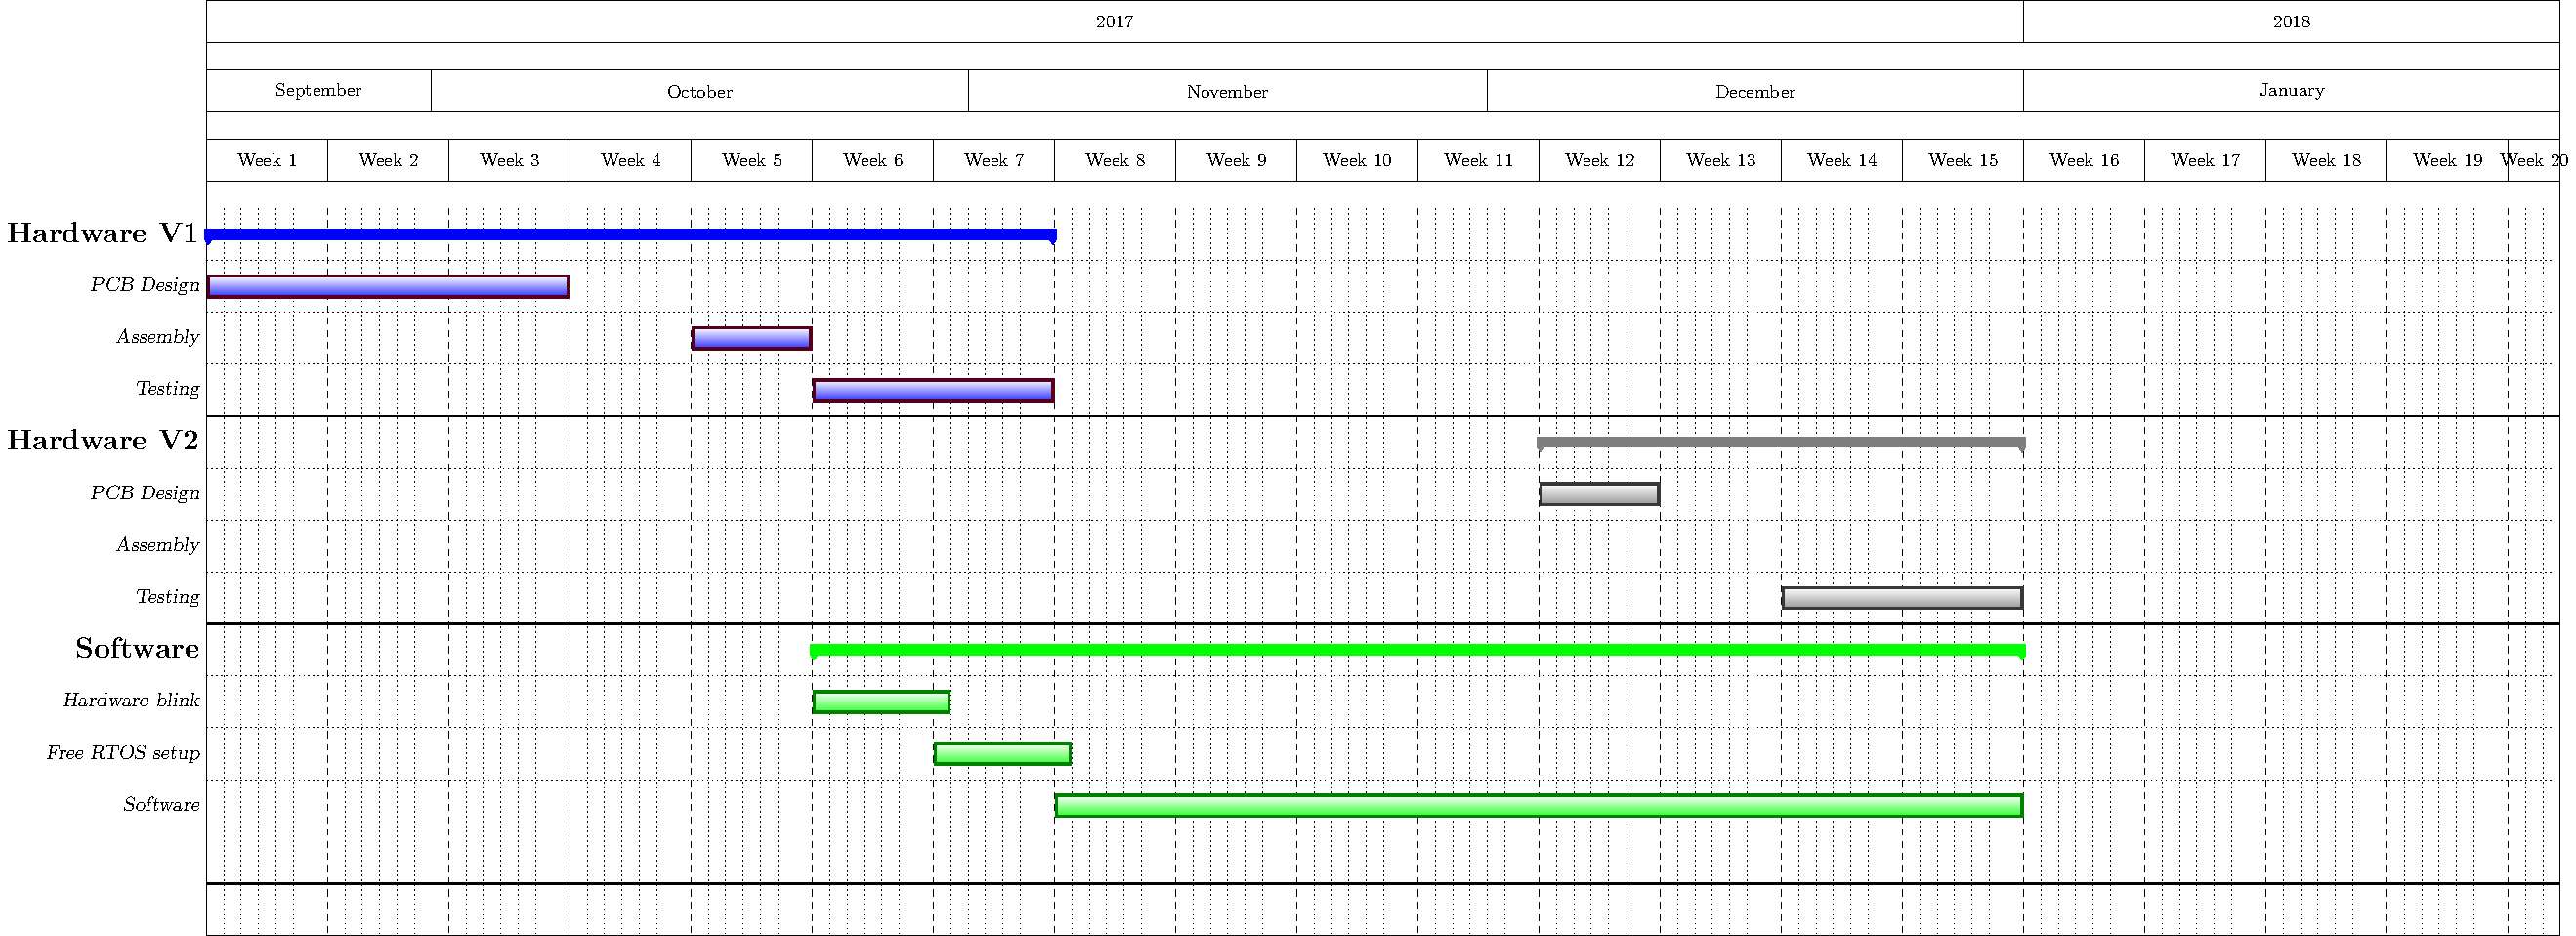
\includegraphics[width=1\textheight, angle=90, origin=c]
    {ProjectPlan_CompleteHwRedesign.pdf}
    \caption{Possible project plan of a complete hardware redesign}
    \label{Project plan complete HW redesign}
\end{figure}
%
\subsection{Adapter Board}
The most profound hardware change is the replacement of the Teensy 3.1.\\
First, a new development board or micro controller has to be selected that supports hardware debugging and meets the requirements for data encryption. \\
After selecting a replacement for the Teensy 3.1, the fastest way to get started with software development for the new micro controller is by designing an adapter board with a Teensy 3.1 footprint. \\
The Teensy 3.1 ships with headers that can be soldered onto the development board. Andreas Albisser designed the interface for the Teensy with female header pins so the development board could simply be plugged into the header and exchanged if needed. This makes it easy to design an adapter print with male headers that match the footprint of the previously used Teensy 3.1. \\
\spic{BareBaseBoard.png}{Base board with female header, Teensy 3.1 not plugged in}{\label{picBareBaseBoard}}
The base board with female headers can be seen in \autoref{picBareBaseBoard}. In this picture, the Teensy 3.1 is not plugged in, the empty headers can be used to route the pins of an other microcontroller to control the base board.\\
This solution has been chosen in the scope of this work to ensure that the end result of this project would provide solid ground work for further development.
%
%
%
\section{Component Evaluation}
Before starting with the design of an adapter board, a replacement for the Teensy 3.1 development board has to be chosen. \\
%
\subsection{Development Board Selection} \label{subsec:txtTeensySelection}
The easiest option is to select a more powerful Teensy development board that meets the requirements listed in appenedix \autoref{app:Aufgabenstellung}.\\
Fortunately, both the Teensy 3.5 and Teensy 3.6 meet the requirements and have an on-board SD card slot. A comparison between the Teensies can be found in \autoref{tableTeensyComparison}
%
\begin{table}[h]
    \begin{center}
        \begin{tabular}{l|L{4cm}L{4cm}L{4cm}}
             & \textbf{Teensy 3.1} & \textbf{Teensy 3.5} & \textbf{Teensy 3.6} \\
             \hline
             %-------------------------------------------------------------------------------------
            \textbf{Processor} & MK20DX256 \newline 32 bit ARM \newline Cortex-M4 \newline 72 MHz & 
            MK64FX512VMD12 \newline Cortex-M4F \newline 120 MHz & 
            MK66FX1M0VMD18 \newline Cortex-M4F \newline 180 MHz \\
            \textbf{Flash Memory [bytes]} & 262 k & 512 k & 1024 k \\
            \textbf{RAM Memory [bytes]} & 65 k & 196 k & 256 k \\
            \textbf{EEPROM [bytes]}	 & 2048 & 4096 & 4096 \\
            \textbf{I/O} & 34, 3.3V, 5V tol & 58, 3.3V, 5V tol & 58, 3.3V, 5V tol \\
            \textbf{Analog In} & 21 & 27 & 25 \\
            \textbf{PWM} & 12 & 17 & 19 \\
            \textbf{UART,I2C,SPI} & 3 & 6 & 6 \\
            \textbf{SD Card} & no & yes & yes \\
            \textbf{Price} & \$19.80 & \$25.25 & \$29.25 \\
        \end{tabular}
    \end{center}
    \stabcaption{Teensy comparison}         
    \label{tableTeensyComparison}
\end{table}
%
The pins of both Teensy 3.5 and 3.6 are backwards compatible to the pin out of Teensy 3.1 which will make it easier to develop the PCB of an adapter board. \\
The Teensy 3.5 and Teensy 3.6 development board have all pins needed for SWD hardware debugging available as pads on their backside. \\
The Teensy 3.5 was chosen for this application because there is more support available for this component and an already configured FreeRTOS. This is not the case with the Teensy 3.6.\\
%
%
\subsection{Preparation for Hardware Debugging}
The Teensy development boards are meant for USB programming and debugging. They are equipped with a small micro controller that acts as a boot loader. The small micro controller is in control of the hardware debugging and reset pins of the main micro controller and does the programming of the main micro controller. This way, all Teensies can be used with standard Arduino libraries and programmed with the Arduino IDE. \\
The schematic of the Teensy 3.5 can be seen in \autoref{picSchematicTeensy3.5}. The MKL02Z32VFG4 acts as the boot loader and the MK64FX512 is the main micro controller.\\
\spic{Teensy35_Schematic.png}{Schematic Teensy 3.5}{\label{picSchematicTeensy3.5}}
\spicv{Teensy35_PinAssignment_FrontSide.png}{Pin assignment, front side}{\label{Pin assignment, front side}}{100}
\spicv{Teensy35_PinAssignment_BackSide.png}{Pin assignment, back side}{\label{Pin assignment, back side}}{100}.\\
The pins available to the user are shown in \autoref{Pin assignment, front side} and \autoref{Pin assignment, back side}. \\
%
\subsubsection{Serial Wire Debug (SWD)}
\spicv{SWD_Pinout.png}{SWD pinout}{\label{SWD pinout}}{70}
As can be seen in \autoref{Pin assignment, back side}, there are SWD (Serial Wire Debug) pins are available as pads on the back side of the Teensy 3.5. \\
The SWD interface consists of the following pins:
\begin{itemize}
    \item Vref: Supply voltage
    \item GND: Ground
    \item SWDIO/DD: Debug Data
    \item SWDCLK/DC: Debug Clock
    \item DE: Debug Enable
    \item RST: Reset
\end{itemize}
The physical pinout of a SWD interface can be seen in \autoref{SWD pinout}. Only the reset, data, clock and ground pins are absolutely required to be connected for the debugging interface to work correctly.\\
Both Teensy 3.5 and Teensy 3.6 have the required SWD pins available on their back side but the debug interface is controlled by the on-board boot loader. \\
There are two ways to communicate to the main micro controller directly without the boot loader interfering on the hardware debugging interface:
\begin{itemize}
    \item Holding the boot loader in reset mode.
    \item Removing the boot loader completely.
\end{itemize}
\subsubsection{Resetting the Boot Loader} \label{txtResettingTheBootLoader}
\spic{Pinout_Bootloader.JPG}{Pin out MKL02Z32VFG4}{\label{picPinoutBootLoader}}
According to the data sheet of the boot loader (see \autoref{picPinoutBootLoader} ), pin 15 of the boot loader can have one of three functions: \\
\begin{itemize}
    \item Reset
    \item GPIO input
    \item GPIO output
\end{itemize}
As default, the pin will be configured as a reset pin, but this function can be turned off by configuring it for any of the other two functions in software. \\
Even though the Teensies are fully open source, the software for the boot loader is not available. The only way to find out if the reset pin is still configured as such is by pulling it low and attempting a reset. \\
The location of the boot loader can be found in \autoref{picBootLoaderHighlighted}.\\
Before putting the boot loader into reset mode, any other functions that this micro controller may be responsible for need to be ensured. \\
Because the internal pull ups of the boot loader are used for the reset line of the main micro controller, this reset line needs to be pulled up externally first. \\
\spic{ResettingBootLoader.jpg}{Trying to pull the boot loader into reset mode}{\label{picPullingBootLoaderResetLow}}
A resistor can be soldered onto the Teensy directly for this purpose as seen in \autoref{picPullingBootLoaderResetLow}. Afterwards, pin 15 of the boot loader can be pulled low. \\
Unfortunately, pin 15 seems to be configured as a GPIO pin because pulling the boot loaders reset line low does not prevent it from communicating to the main micro controller of the Teensy 3.5. \\
\spic{Teensy35_uC_keeps_Talking_Even_with_RESET_pulled_to_3V3.png}{The boot loader keeps communicating to the Teensy}{\label{picBootloaderKeepsTalking}}
The state of the hardware debugging pins during idle state were checked with the scope but as can be seen from \autoref{picBootloaderKeepsTalking}, the boot loader is still in control of the debugging interface and therefore the main micro controller.\\
Instead of investigating further into this option, the second option was chosen. \\
%
\subsubsection{Removing the Boot Loader} \label{txtRemovingTheBootLoader}
The MKL02Z32VFG4 has two functions:
\begin{itemize}
    \item It acts as a boot loader and controls the SWD interface to the main micro controller.
    \item It controls the reset line of the main micro controller and its internal pull ups are used to keep the reset line in idle state.
\end{itemize}
To leave the user in full control of the SWD hardware debugging interface, the boot loader has to be removed (or silenced, as attempted in \ref{txtResettingTheBootLoader}). \\
\spicv{BootLoaderHighlighted.png}{Location of the bootloader on Teensy 3.5}{\label{picBootLoaderHighlighted}}{100}
The MKL02Z32VFG4 is located on the front side of the Teensy, as indicated in \autoref{picBootLoaderHighlighted}.\\
\spicv{Teensy35_Modified.png}{Teensy 3.5 modified for hardware debugging}{\label{picModifiedTeensy}}{100}
Flux gel was applied around the boot loader before heating the soldering pads up with hot air to remove the MKL02Z32VFG4. Now a pull up resister was added as seen in \autoref{picModifiedTeensy}. Afterwards, the SWD debugging interface could be used. \\
%
%
%
%
%
%
\section{Teensy Adapter Board} \label{sec:txtTeensyAdapterBoard}
The design of the adapter board from the footprint of the Teensy 3.1 to the footprint of the Teensy 3.5 was straight forward because of backwards compatibility of the pinout.\\
The Teensy 3.5 is slightly longer than the Teensy 3.1 so the extra pins of the newer version will not be routed down to the main board. The backwards compatible pins can be used like before.\\
Additional components for the adapter board include:
\begin{itemize}
    \item Hardware debugging interface.
    \item Pull up resistor for reset line
    \item Ground header
    \item 3.3V header
\end{itemize}
To prepare the Teensy 3.5 for usage within this project, male headers have to be soldered onto the board and the boot loader has to be removed as in \ref{txtRemovingTheBootLoader}. Because the reset line will be pulled up to 3.3V on the adapter board, the on-board pull up resistor (as seen in \autoref{picModifiedTeensy}) for the reset line is optional. It is only required when working with the Teensy 3.5 stand-alone without the adapter board.\\
Schematic and PCB of the Teensy adapter board can be found in the appendix \todo{Link zum Schema+PCB vom Adapter Board im Appendix}.\\
Issues encountered during development of the adapter board were the pin numbering and interlayer connections.
\subsubsection{Pin numbering}
In a first version of the Teensy adapter board, the pin numbering of the SWD debugging connector was done wrong and had to be adjusted in the footprint for a next PCB version.\\
\spic{DebuggingWithWrongFootprint.jpg}{Hardware debugging with faulty SWD footprint}{\label{fig:picDebugSetupWrongAdapterBoard}}
But instead of waiting for the next PCB version to be produced, all debugging signals were routed manually from the faulty SWD pinout to the debugger. This way, development of the software could be started without delay. A picture of the signal routing can be seen in \autoref{fig:picDebugSetupWrongAdapterBoard}.
\subsubsection{Interlayer connections}
The next PCB ordered for internal production at HSLU had poor interlayer connections, most vias did not connect through.\\
To verify the changes on the SWD pinout, the relevant debugging pins were routed manually with small wires and they seem to be correct.\\
But for simplicity and time reasons, not all signals were routed manually but an other order was placed at the HSLU internal production with the hope of better interlayer connections but again with insufficient result.\\
Only on the third HSLU internal order, the inter connection seemed to be satisfying.\\
But by then, there was not enough time to assemble and test the produced adapter boards.\\
%
%
%
%
%
%
%